\documentclass[12pt]{article}
% Эта строка — комментарий, она не будет показана в выходном файле
\usepackage{ucs}
\usepackage[warn]{mathtext}
\usepackage[utf8x]{inputenc} % Включаем поддержку UTF8
\usepackage[russian]{babel}  % Включаем пакет для поддержки русского языка
\usepackage{amsmath}
\usepackage{mathtools}
\usepackage{amssymb}
% \usepackage[dvips]{graphicx}
% \graphicspath{{noiseimages/}}
\usepackage[pdftex]{graphicx}


% Параметры страницы: 1см от правого края и 2см от остальных.


\hoffset=0mm
\voffset=0mm
\textwidth=180mm        % ширина текста
\oddsidemargin=-6.5mm   % левое поле 25.4 - 5.4 = 20 мм
\textheight=240mm       % высота текста 297 (A4) - 40
\topmargin=-15.4mm      % верхнее поле (10мм)
\headheight=5mm      % место для колонтитула
\headsep=5mm          % отступ после колонтитула
\footskip=8mm         % отступ до нижнего колонтитула


\begin{document}
    \author {Жарков Андрей 496}
    \title {Лабораторная работа 1.3 \\  Изучение колебаний на примере физического маятника}
    \maketitle{}   

    \indent
    \textbf{Цель работы:} исследовать физический и математический маятники
    как колебательные системы, измерить зависимость периода колебаний физического маятника от его момента инерции.
    \\ \\
    \indent
    \textbf{В работе используются:} физический маятник (однородный стальной стержень), опорная призма, математический маятник, счётчик числа колебаний, линейка, секундомер.
    \\
    Физическим маятником называется любое твёрдое тело, подвешенное на неподвижной горизонтальной оси и совершающее колебательное движение под действием возвращающих сил (рис. 1). В рассматриваемом случае возвращающей силой является сила тяжести. \\ \\
    
    \begin{center} 
    	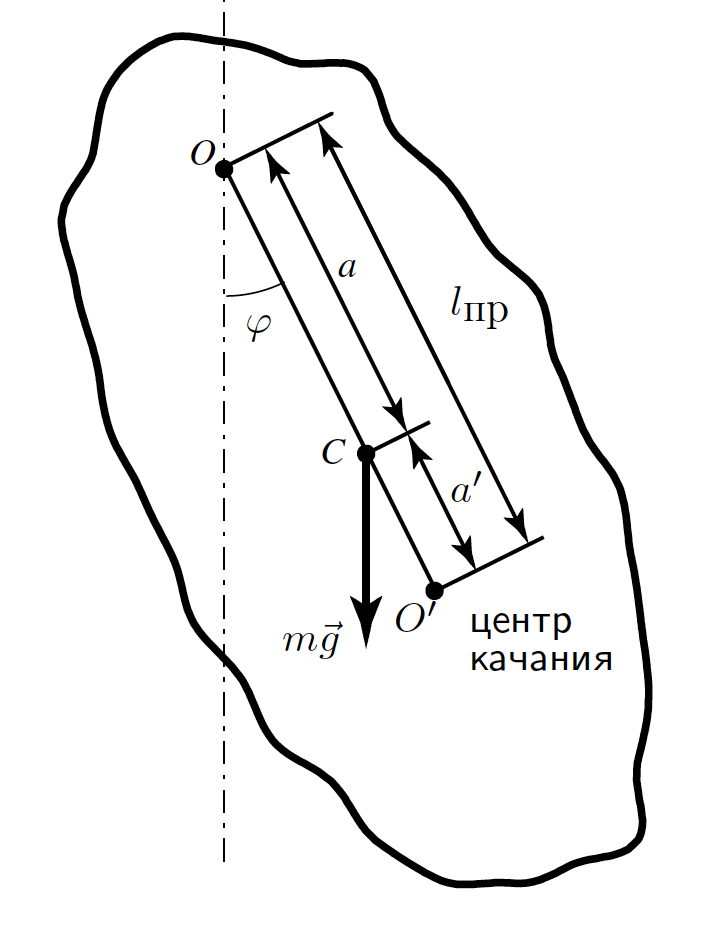
\includegraphics[width=1.5in]{phys_mtn.png} \\ Рис. 1: физический маятник.
    \end{center}
    
    Колебания маятника в свою очередь представляют частный случай вращательного
    движения твёрдого тела вокруг неподвижной оси. При устойчивом равновесии центр масс маятника лежит на одной вертикали с точкой подвеса ниже её. При колебаниях прямая, соединяющая точку подвеса с центром масс,
    отклоняется от вертикали на угол $\phi$. Если зависимость этого угла от времени $\phi$(t) будет
    определена, то мы получим точное математическое описание колебаний физического маятника. Следовательно, для
    анализа особенностей движения маятника можно использовать основное уравнение вращательного движения относительно оси, проходящей
    через точку подвеса 𝑂 перпендикулярно к плоскости рисунка:
    \begin{equation}
       I \ddot \phi = M
    \end{equation}
	
    где 𝐼 — момент инерции маятника относительно оси вращения, 𝑀 —
    суммарный момент всех сил, действующих на маятник. В пренебрежении силами трения 𝑀 равен моменту силы тяжести, которая приложена к центру масс маятника: 
    \begin{equation}
       𝑀 = −𝑚g𝑎 \sin\phi.
    \end{equation}
    Здесь 𝑚 — масса маятника, 𝑔 – ускорение свободного падения, 𝑎 — расстояние от точки подвеса 𝑂 до положения центра масс 𝐶. Если в процессе колебаний угол $\phi$(𝑡) всегда мал, то $\sin\phi \approx \phi$ и можно приближённо записать
    \begin{equation}
       𝑀 \approx −𝑚g𝑎\phi.
    \end{equation}
    Тогда уравнение (1) с учётом (3) принимает вид
    \begin{equation}
        𝐼\ddot{\phi} + 𝑚g𝑎\phi = 0.
    \end{equation}
    
    Полученное уравнение есть уравнение гармонических колебаний. Пере-
    пишем его в стандартном виде:
    \begin{equation}
       \ddot{\phi} + \omega_0^2\phi = 0,
    \end{equation}
    где
    \begin{equation}
    \omega_0 = \sqrt{\frac{mga}{I}}
    \end{equation}
    — циклическая частота колебаний маятника. \\
    Решением (5) является функция вида
    \begin{equation}
    \phi(t) = Asin(\omega_0 + \alpha)
    \end{equation}
    Амплитуда колебаний 𝐴 (максимальный угол отклонения) и начальная
    фаза $\alpha$ определяются начальными условиями задачи. Период колебаний,
    легко измеряемый на практике, равен
    \begin{equation}
    T = \frac{2\pi}{\omega_0} = 2\pi\sqrt{\frac{mga}{I}}
    \end{equation}
    Если размер тела намного меньше длины (невесомого) подвеса 𝑙, то
    такое тело можно считать точечной массой (материальной точкой), а
    маятник математическим. В этом случае $𝐼 = 𝑚𝑙^2$ и 𝑎 = 𝑙. Поэтому
    период колебаний математического маятника равен
    \begin{equation}
    T_{мат} = 2\pi\sqrt{\frac{l}{g}}
    \end{equation}
    
    Длину математического маятника, период колебаний которого равен
    периоду колебаний данного физического маятника, называют приведённой:
    \begin{equation}
    l_{пр} = {\frac{I}{ma}}
    \end{equation}
    Точку, находящуюся на расстоянии $𝑙_{пр}$ от точки подвеса вдоль линии,
    проходящей через центр масс (точка 𝑂′ на рис. 1), называют центром
    качания. Если перевернуть физический маятник, подвесив его за центр
    качания, то приведённая длина, а значит, и период колебаний не изме-
    нятся, при этом старая точка подвеса 𝑂 станет новым центром качания.
    
    % ДОБАВИТЬ ТЕОРИЮ

    \textbf{Экспериментальная установка.}
    В данной работе в качестве физического маятника используется однородный стальной стержень длиной
    $l$  На стержне закрепляется опорная призма, острое ребро
    которой является осью качания маятника. Призму можно перемещать
    вдоль стержня, меняя расстояние $a$ от точки опоры (точки подвеса)
    маятника до его центра масс. Используя теорему Гюйгенса–Штейнера 
    и считая стержень тонким (его радиус много
    меньше длины), вычислим его момент инерции: $$I = \frac{ml^2}{12} + ma^2$$
    \\
    Тогда, подставляя это выражение в формулы (8) и (10), получим основные характеристики используемого маятника — период его колебаний
    и приведённую длину:
    \begin{equation}
    T = 2\pi\sqrt{\frac{a^2+\frac{l^2}{12}}{ag}}
    \end{equation}
    \begin{equation}
    l_{пр} = a+\frac{l^2}{12a}
    \end{equation}
    Величину 𝑎, входящую в (11), и положение точки подвеса можно изменять с помощью передвижной опорной призмы. Также можно сравнить приведённую длину маятника, вычисленную по формуле (12), с
    длиной математического маятника. В данной работе в качестве математического маятника используется свинцовый шарик, подвешенный на двух расходящихся нитях. Длину нитей можно изменять, наматывая их
    на ось (рис. 3).
    \begin{center} 
    	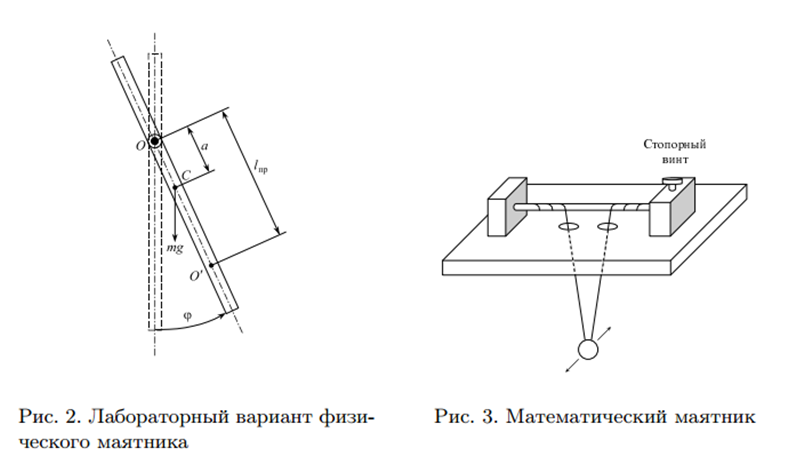
\includegraphics[width=5in]{lab3_2.png}.
    \end{center}
    \pagebreak
    \textbf{\large Выполнение работы} \\\\
    \textbf{Вычисление погрешностей}
       \begin{table}[ht]
       	\caption{измерения вермени 25 периодов физического маятника}
       	\begin{center}
       		\begin{tabular}{|c|c|c|c|c|c|}
       			\hline 
       			$i$ & 1 & 2 & 3 & 4 & 5 \\
       			\hline
       			$t_i$,c & 38.48 & 39.04 & 38.85 & 38.89 & 38.80 \\
       			\hline
       		\end{tabular}
       	\end{center}
       \end{table}
       
       $\sigma_{отд} = \sqrt{\frac{\Sigma (t_i - t_{cp})^2 }{n-1}} \approx 0.2 c$ \\
       $T_{ср} = 1.552 \pm 0.008 с$ \\
       
       \begin{table}[ht]
       	\caption{измерения вермени 25 периодов математического маятника}
       	\begin{center}
       		\begin{tabular}{|c|c|c|c|c|c|}
       			\hline 
       			$i$ & 1 & 2 & 3 & 4 & 5 \\
       			\hline
       			$t_i$,c & 29.90 & 30.36 & 30.13 & 30.00 & 30.27 \\
       			\hline
       		\end{tabular}
       	\end{center}
       \end{table}
       
       $\sigma_{отд} = \sqrt{\frac{\Sigma (t_i - t_{cp})^2 }{n-1}} \approx 0.19 c$ \\
       $T_{ср} = 1.205 \pm 0.007 с$ \\   
       
    \textbf{Проверка допустимости предположений} \\ \\
       Для физического маятника время уменьшения амплитуды в 2 раза $\tau_2$ = 247 c, откуда \\
       $\tau_e = \frac{-1}{ln\frac{1}{2}} \tau_2 = 355 c >> T$ \\
       $Q_{физ}=\pi \frac{\tau_e}{T}$ = 720 \\
       Проверим незначительность зависимости периода от амплитуды \\
       $\alpha = 30^\circ$ T = 1.600 $\pm$ 0.008 c \\
       $\alpha = 15^\circ$ T = 1.589 $\pm$ 0.008 c \\
       $\alpha = 5^\circ$ T = 1.596 $\pm$ 0.008 c \\ \\
       
       Для математического маятника время уменьшения амплитуды в 2 раза $\tau_2$ = 291 c, откуда \\
       $\tau_e = \frac{-1}{ln\frac{1}{2}} \tau_2 = 419 c >> T$ \\
       $Q_{мат}=\pi \frac{\tau_e}{T}$ = 1094 \\ \\
       
    \textbf{Проверка обратимости} \\ \\
       При положении, когда стержень подвешен на расстоянии 47 см (длинна маятника 1 м) от центра тяжести T = 1,612 $\pm$ 0.008 c, соответствующе подобранная длинна математического маятника $l_{мат}$ = 64,5 см. $T_{мат}$ = 1.614 $\pm$ 0.007 c. Получилось так, что найденная $l_{мат}$ точно совпала с теоретически рассчитанной по формуле (12) - 
       $l_{мат}^{теор}$ = 64.5 см \\ \\
       
       $l_{обр} = l_{пр} - a = 17.5 см$ \\
       $T_{обр} = 1.612 \pm 0.008 с$ \\
       Как видим, в пределах погрешности обратимость подтверждена. \\
       
    \textbf{Зависимость периода колебаний 𝑇 от расстояния 𝑎 между точкой опоры и центром масс.} \\
     При измерении $\sigma_a = 0.5sm$, $\sigma_T = 0.008sec$. \\
     
     \begin{center} 
     	результаты измерений  \\
     	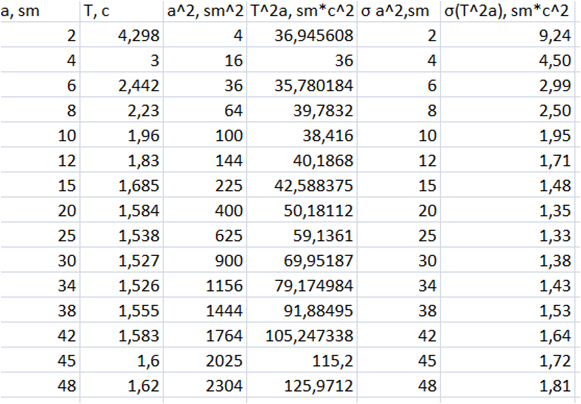
\includegraphics[width=3.5in]{lab3_table.png}
     	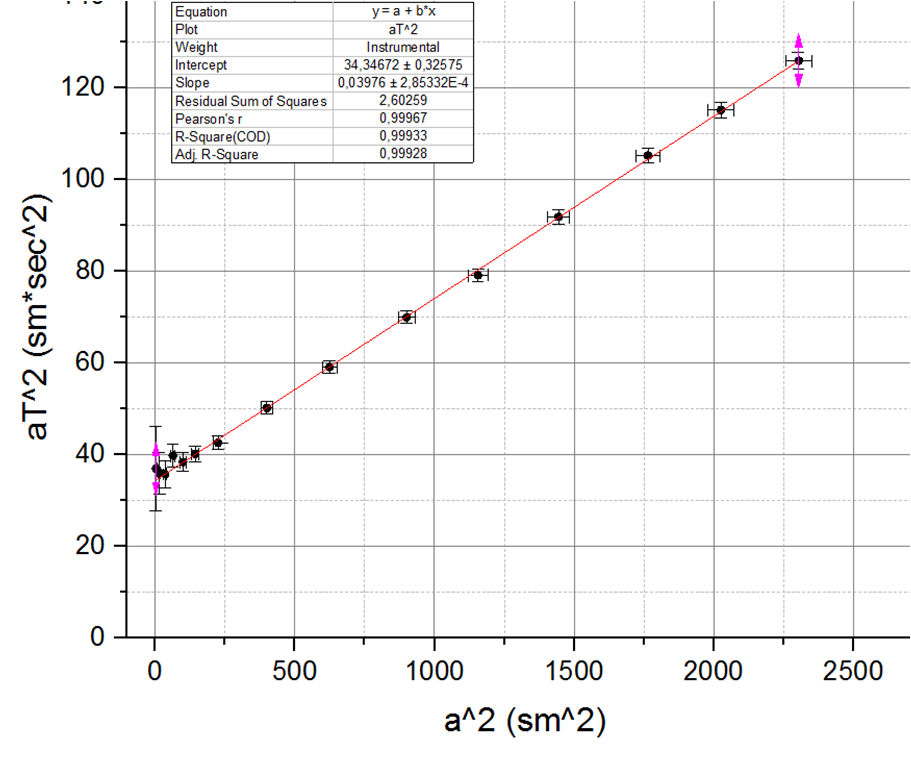
\includegraphics[width=5.5in]{lab3_plot.png}
     \end{center}
     
     Отсюда $T^2a = ka^2+b$, где k = 3.97 $\pm$ 0.03 $c^2$/м, b = 34.3 $\pm$ 0.3см*$c^2$ \\
     
     Уравнение (11) перепишем в виде $$T^2a=\frac{4\pi^2}{g}a^2+\frac{4\pi^2}{g}\frac{l^2}{12}$$
     Тогда g=$\frac{4\pi^2}{k}$=9.94 $\pm$ 0.08 м*$с^2$ \\
     l = $\sqrt{\frac{12b}{k}}$ = 1.01 $\pm$ 0.01 м \\
     Как видим, с хорошей точностью, это совпадает с табличными значениями.
       
\end{document}